\documentclass{article}
\usepackage{relsize}
\usepackage{tikz} % ,pgf,pgfarrows,pgfnodes,pgfautomata,pgfheaps,pgfshade}
\usetikzlibrary{shapes,decorations,shadings,positioning,arrows}
\usepackage{amsmath,enumerate,xspace}
\usepackage{listings}
\usepackage[absolute,overlay]{textpos}

\usepackage[colorlinks=true,linkcolor=red,pagecolor=red,
  citecolor=blue,urlcolor=blue,breaklinks=true,
  hyperfootnotes=false,pdftitle={CombLayer Guide},
  pdfauthor={Stuart Ansell},pdfkeywords={CombLayer,MCNP,MCNPX}]
           {hyperref}
\renewcommand*{\rmdefault}{cmss} 

\newcommand{\cinder}{{\tt CINDER}\xspace}


\newcommand {\prog}[1]{{\it #1}}
\newcommand {\vb}[1]{\begin{\verbatim}{#1}\end{verbatim}}


\title{CombLayer Guide}
\author{Stuart Ansell}

\begin{document}
\maketitle
\tableofcontents

\section{Introduction}

CombLayer is designed to facilitate the rapid production of complex
MCNP(X) models that depend on a long list of ranged variables and a
number of module flags. It is also intended to help with placement of tallies,
maintaining consistant material files and some variance reduction.

\subsection{Coding Convensions}

CombLayer has some coding convensions beyond the standard Scott Myers
Efficient C++ convensions \cite{Myers}. These are typcially there for
two reasons (i) that in a model-build system, a rapid build time is
essential since it is nearly impossible to have a sub-test framework for any
component as the whole MCNP(X) model is required to check if is it
valid, (ii) the code is intended to be used without complete
understanding. Therefore as much as possible, each component is
independent without code repetition. Back-references are to be minimized
both in the run-time calling path and in the code build dependencies.

\subsubsection{Include files}
\label{Sec:IntroInclude}
Include files (.h) are forbidden to include other files.
This does several things (a) it reduces the {\it dependency
  hell} where it is almost impossible to find the definition of a
function and what it depends on. (b) optimization of the include tree
can be carried out and dependency continuously observered. 

Namespaces are a good method of removing global name pollution but
many other C++ programs allows {\it using namespace X}, this is almost
100\% forbidden except in the test for that particular namespace
unit. This also applies to boost, stl, tr1 etc, to which helps
distinguish external functions and domains.



\newpage
The basic program structure is 

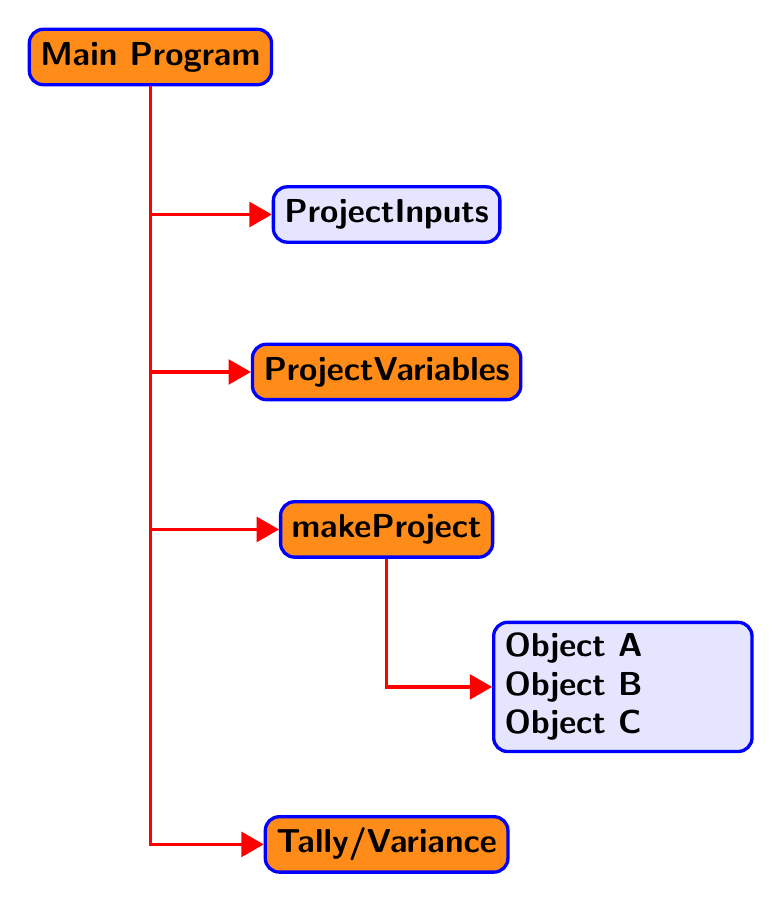
\begin{tikzpicture}

  \coordinate (Main) at (0,0);
  \coordinate (Input) at (3,-2);
  \coordinate (Var) at (3,-4);
  \coordinate (Project) at (3,-6);
  \coordinate (Object) at (6,-8);
  \coordinate (Tally) at (3,-10);

  \tikzstyle{fbox}=[draw=blue,very thick,
                    shape=rectangle,rounded corners=0.5em,
                    inner sep=4pt,
                    minimum height=2em,text badly centered,
                    fill=orange!90!white];
  \tikzstyle{obox}=[draw=blue,very thick,
                    shape=rectangle,rounded corners=0.5em,
                    inner sep=4pt,
                    minimum height=2em,text badly centered,
                    fill=blue!10];

%  \draw[blue,line width=0.4mm,->] (tally) (tally) -- (weight);
%  \draw[blue,line width=0.4mm,->] (tally) (geom) -- (weight);
%  \draw[blue,line width=0.4mm,->] (tally) (var) -- (geom);
%  \draw[blue,line width=0.4mm,dashed,->] (tally) -- (geom);


  \node[fbox] (MainBox) at (Main) { \bf \large Main Program } ;

  \node[obox] (InputBox) at (Input) { \bf \large ProjectInputs };
  \draw[->,very thick,color=red,>=triangle 60] (MainBox) |- 
                   node[left]{} (InputBox) ;

  \node[fbox] (VarBox) at (Var) { \bf \large ProjectVariables };
  \draw[->,very thick,color=red,>=triangle 60] (MainBox) |- 
                   node[left]{} (VarBox) ;

  \node[fbox] (ProjectBox) at (Project) { \bf \large makeProject };
  \draw[->,very thick,color=red,>=triangle 60] (MainBox) |- 
                   node[left]{} (ProjectBox) ;

  \node[obox] (ObjectBox) at (Object) { \parbox{3.0cm}{ \bf \large Object A\\
 Object B\\ Object C} };
  \draw[->,very thick,color=red,>=triangle 60] (ProjectBox) |- 
                   node[left]{} (ObjectBox) ;

  \node[fbox] (TallyBox) at (Tally) { \bf \large Tally/Variance };
  \draw[->,very thick,color=red,>=triangle 60] (MainBox) |- 
                   node[left]{} (TallyBox) ;

%  \shade[left color=blue!50,line width=0.5cm] (3,1.5) circle (2.0cm);
%  \shade[left color=red,line width=0.5cm] (var) circle (1.30cm);
%  \shade[left color=green,line width=0.5cm] (tally) circle (1.30cm);

%  \node at (weight) { {\bf \large Variance} };
%  \node at (var) { {\bf \large Variables} };
%  \node at (tally) { {\bf \large Tallies} };



%\node
\end{tikzpicture}


\section{Installation}

CombLayer is predominately written for the Linux platform using {\tt C++}
compilers that support {\tt C++11} or greater. The code is available from \\
\href{https://github.com/SAnsell/CombLayer}{https://github.com/SAnsell/CombLayer}, \\ either as a download of a {\tt zip} file or
by cloning/pulling the git repository.

\subsection{Requirments}

CombLayer needs to have the GNU Scietific Library [GSL] and the
{\tt boost::regex} system along with the STL libraries from your {\tt C++}
compiler. The GSL can be avoided with the {\tt -NS} flag in the {\tt getMk.pl} \checkme{or CMake.pl?} script
but some functionality will be lost, particularly in the choice
of variance reduction methods.

Additionally, the primary build system uses {\tt cmake}. There is another
that just uses {\tt make} but is significantly more time-consuming.

Functional documentation is supported using {\tt Doxygen} and the construction
of new cmake text files can be done via PERL scripts.

Currenly it is know that {\tt gcc} version 4.6 and above can compile
CombLayer as can {\tt clang} (all tested versions). {\tt gcc} 4.4 which is often
the default on RedHat systems (2015) does not work.

\subsection{Basic build method}

If a clean directory is made and then the {\tt .zip} file is uncompressed, the
following commands should build a version of CombLayer.

\begin{bash}
  ./CMake.pl
  cmake ./
  make
\end{bash}

This should make a number of executables, e.g. {\tt ess}, {\tt simple}, {\tt fullBuild} etc. These
can be used to make a simple model with commands like
\begin{bash}
  ./simple -r AA
\end{bash}
This will produce an output file {\tt AA1.x} which is a MCNP model.




\section{Link system}

CombLayers geometry is composed of a set of objects that have slightly
stronger rules than a typical MCNPX model. Obviously any MCNPX model
can be represented as a CombLayer model and in the extreme case that
is done by defining one object to contain the MCNPX model. However, the
little benefit would be derived from such an approach.

The basic geometric system is to build a number of geometric classes
and construct the model by incorporating those into the desired
configuration. Each geometric class is designed to be built and an
arbitary position and rotation, be of an undetermined number, and
interact with its surroundings in a well defined manor. 

In object orientated programming, functional rules and properties are
normally added to objects by inherritance. CombLayer follows that
pattern. As such most geometry item classes inherit from base classes within 
the {\tt attachSystem} namespace.

\subsection{AttachSystem Namespace}
\label{AttachSystem}

The CombLayer system is built around the interaction of FixedComp
units, ContainedComp units and LinkUnits. The use of these and their
interactions are the basic geometric building tools. These object
reside within the attachSystem namespace.

Almost any geometric item can be designated as a FixedComp
object. This is done by public inherriting from directly from the
FixedComp, or by inherriting from one of the more specialised attachSystem
objects e.g. TwinComp or LinearComp. 

\subsection{FixedComp}

The basic FixedComp object holds the origin and the orthoganal basis
set (X/Y/Z) for the geometry item being built. In addition it holds a 
number of LinkUnits which provide information about the outer (and/or inner)
surfaces and positions on the geometric item. 

As with all Object-Orientated (OO) constructions their is an implicit
contract that the inherited object should adhere to. This is normally
expressed as the {\it Liskov Substitution principle}: This principle
states that functions that use pointers/references to the base object
must be able to use the objects of derived classes without knowing
it. In this case, that means that modification of the origin or the
basis set should not invalidate it and that the object should do the
expected thing. E.g. if the origin is shifted by 10 cm in the X
direction the object should move by 10cm in the X direction. It also
means that the basis set must remain orthogonal at all time.

Other than providing an origin and an basis set, the FixedComp has a
number of link points. The link points are there to define joining
surfaces, points and directions. Each link point defines all three parts.

For example a cube might have 6 linkUnits, and each linkUnit would
have a point at the centre of a face, a direction that is normal to
the face pointing outwards and a surface definition that is the
surface pointing outwards. [ Note that in the case that the link
points define an inner volume, for example in a vacuum vessel, then
the surfaces/normals should point towards the centre.]

The actual link surface does not need to be a simple surface. In the
case, that an external surface needs multiple surfaces to define the
external contact these can be entered into a link-rule. For example,
if the cube above was replaces with a box with two cylindrical
surfaces the link surface would be defined as the out going cylinder
intersection with a plane choosing the side. 

In the case of an equiry for the linkSurface (e.g. to do an line
intersection) then it is the first surface that takes
presidence. However, all actions can be carried out on the link-rule
including line intersections etc.


\subsection{ContainedComp}

The ContainedComp defined both the external and interal enclosed
volume of the geometric item. It is most often used to exclude the
item from a larger enclosing geometric object: e.g. A moderator will
be excluded from a reflector, or it can be used to exclude a part of
the geometric item from another geometric object. E.g. two pipes which
overlap can have one exclude itself from the other. 

In CombLayer, the ContainedComp are considered the primary geometric
item, i.e. it is the ContainedComp that is removed from the other
items.  However, it is used in a two stage process wereby cells are
registered to be updated by the ContainedComp at a later date. This
was to allow forward dependency planning but has more or less been
superseded by the attachControl system.


\section{Model Runtime control}

C++ programs start from the main() function and in CombLayer the
runtime control has been keep mostly in the main() function. Clearly
that could be further refactored out but CombLayer lacks the
sophisticated top level type abstraction that is required to do this
in a generic way, so copy/pasted structure is used with variance to
the particular model required. The sole advantage of the abscence of a
top level abstraction is that the user is the freedom in writing new objects
which allows other programs to be incorporated by making their main function
a minor function and directly calling.

The structure of two example main()s will be compared from the units
that exist with the stanard CombLayer distribution. That is {\it
bilbau.cxx} and {\it reactor.cxx}. These build the delft reactor model and the
Biblau low energy spallation source.

First part of the code is along list of \#include's. They are the
mainly dependency list of the objects {\it Simulation, weightManager,
and tallySelector.} This can and should be copied at will. Do not
make an file with them all in [see \ref{Sec:IntroInclude}].

At the end of the include section there is typically, one or two model
specific includes. These normally include {\it makeXXX.h} file and
anything that they directly depend on. In the case of bilbau it is just 
{\it makeBib.h} whilst for reactor it is both {\it makeDelft.h} and \prog{ReactorGrid.h}.

\subsection{makeModel}

The makeModel object is the place that creates, initializes and
manages inquires for the instances of all the geometric components. 
Primary objects need to be created and registered with the objectRegister 
\ref{objectRegister}. The makeModel component is 
 




Tallies are the fundamental reason for running MCNPX. However, the
manor in which MCNPX specifies tallies is not compatible with a
vairiable defined model because in most cases the required tally is relative 
to an object whose position is unknown. 

This problem has been addressed by allowing most tallies to use the 
FixedComp link system. 

\subsection{Tally System}

The tally system is accessed either by a simple command line menu
system, or via an XML file. The command line help system is very
primative but can remind the user of the bais

\subsection{Point Tally}
\label{PointTally}

Point tallies are fundamentally a 3D vector in space. In CombLayer,
there are three levels of position available: (a) Real MCNPX output
position, (b) CombLayer master origin position before master rotation,
and (c) relative position to an object. Both (a) and (c) are well
supported, however, to do option (b) there needs to be some real care
with the layout of the calling sequence in the main() function. The
fullBuild.cxx example is a suitable option to follow, but checking
will be needed.

As


\section{Components}

\section{ObjectRegister}
\label{ObjectRegister}

The objectRegister is a singleton object [it should be per
  simulation], which keeps each and then deletes when at its lifetime
end, each object registered with it. It only accepts two types of
object, a dummy name object and a FixedComp object. 

If a dummy object is required, the name (and possibly number) of the object 
is provided and the objectRegister singleton provides a unique
range of cell and surface numbers, typically 10,000 units of each, but
can be user selected. This is its only responsibility and to ensure that the
name is unique. 

Significantly more complex is the FixedComp registration, in this case
a \prog{boost::shared\_ptr} of FixedComp must be provided by the
calling method. Obviously, for a shared\_ptr the object memory must be
allocated, i.e. an initial \vb{new object(...)} is normally called
directly or previously. A typical structrue might be:

\begin{verbatim}
boost::shared_ptr<BeamPipe> A 
   = new BeamPipe("LongPipe");

ModelSupport::objectRegister& OR=
    ModelSupport::objectRegister::Instance();

OR.addObject(A);
\end{verbatim}

From this example, the BeamPipe class is inherrited from FixedComp,
this is manditory. A tempory reference \prog{OR} is created by calling
the static Instance() method. All singletons in CombLayer provide an
Instance() method for this purpose. Then the object pointer is referenced
to the objectRegiste with \prog{addObject}.

However, hidden from view is a call to objectRegister in FixedComp's
constructor, which must be called as all registered object must derive
from this class. That occures during the operator new call and results
in the allocation of the cell/surface numerical range. If it is
necessary to trap that error, the try/catch block must be around the
new opertor.





\subsection{EXT Command}

MCNP(X) provides the EXT card for biasing the direction of the
particles after collisions. The card can be configured with a
stretching parameter value between -1.0 and 1.0 and an optional vector
or direction associated with it. If a vector is not given the
stretching parameter is applied in the direction of the neutron travel.

MCNP(X) only accepts the direction to be X,Y,Z which is highly
limiting in the CombLayer environment, so it is only partially supported.

The other two options vector and non-vector are supported.

\subsection{-wExt entry}

The first method of entry is via the command line option -wExt. This
command takes a sequence of additional values which are split into a
{\it zone} and {\it type} region. The {\it zone} region is based on
the cells that are to be biased. This can be give with the commands:

\begin{itemize}
\item{ {\bf all} : Apply to all non-void cells.}
\item{ {\bf Object [name]} : Apply to all objects within the object name.}
\item{ {\bf Cells [N1 N2...]} : Apply to given cell numbers [pre-renumber].}
\item{ {\bf Range [N1  N2]} : Apply to all cell numbers between N1 and N2.}
\end{itemize}

The {\it type} section depends on the type of EXT command required. The options are

\begin{itemize}
\item{ {\bf simple} : Simple $\Sigma_C/\Sigma_T$ scaling.}
\item{ {\bf simpleVec [Vec]} : Simple $\Sigma_C/\Sigma_T$ scaling.} 
\item{ {\bf Object [name]} : Apply to all objects within the object name.}
\item{ {\bf Cells [N1 N2...]} : Apply to given cell numbers [pre-renumber].}
\item{ {\bf Range [N1  N2]} : Apply to all cell numbers between N1 and N2. } 
\end{itemize}




\section{HowTo}
%\section{HowTo}
\begin{itemize}
\item Get real surface number by its relative number: SMap.realSurf(divIndex+103) (see createLinks methods)
\end{itemize}

\subsection{How to put one object into another}

Suppose, we are inserting Spoon into Mug.
Mug is made up of N cells. Spoon is made of one contained component with outer surface.
CombLayer provides several methods to put one object into another:

\begin{lstlisting}[language=C++]{Name=essBuild}{floatplacement=H}
attachSystem::addToInsertForced(System,   *Mug, *Spoon);
attachSystem::addToInsertSurfCtrl(System, *Mug, *Spoon);
attachSystem::addToInsertControl(System,  *Mug, *Spoon);
attachSystem::addToInsertLineCtrl(System, *Mug, *Spoon);
\end{lstlisting}

\subsubsection{addToInsertForced}
The outer surface of the Spoon is excluded from the HeadRule of every single cell of Mug.
Even if Mug contains cells which do not intersect with Spoon (e.g. its handle).
``Forced'' means ``do it and do not think about it'', but at the same time it means that ``I have got something wrong somewhere in my mental thinking''.

\subsubsection{addToInsertSurfCtrl}
First, it deconvolves Mug into its surfaces.
Then for each cell of Mug it calculates intersections between all surfaces of this cell and all surfaces of Mug.
The Mug is inserted only into those cells of Mug which it intersects.

It is not always better to call {\tt addToInsertSurfCtrl} instead of {\tt addToInsertForced}. \alert{Example needed.}

{\tt addToInsertSurfCtrl} is a very expensive function to call, because you have to check all the surface triplets. So, it runs a bit slower than addToInsertForced, but the geometry will be faster.
However, there is another method which provides the same trick for less pain.

\subsubsection{addToInsertControl}
It's a very simple method. Spoon has to have the link points defined.
The method checks if any of these link point fit inside the outer surface of Mug. If it does, then it cuts Spoon from the Mug.
It is possible to add a vector of link points to check as a parameter.

\subsubsection{addToInsertLineCtrl}
Imagine we have a (big) contained component~(Mug) and some (small) object which clips it~(Spoon). The link points are {\bf not} in the Mug~(therefore {\bf addToInsertControl} can not be used), but the lines which connect them are in the Mug.
The method checks the lines connecting the link points and sorts out the intersections.

\end{document}


\end{document}
